\documentclass[conference]{IEEEtran}
\IEEEoverridecommandlockouts

%% ---------------------------------------------------------------------------
%% IEEE conference format (IEEEtran). Bibliography: references.bib.
%%
%% Build:  pdflatex main && bibtex main && pdflatex main && pdflatex main
%%
%% Both figures are drawn in TikZ below, so the paper builds with no external
%% image files. The draw.io sources in figures/ are kept for reference only.
%% ---------------------------------------------------------------------------

\usepackage{cite}
\usepackage{amsmath,amssymb}
\usepackage{makecell}
\usepackage{pifont}
\usepackage{url}
\usepackage{tikz}
\usetikzlibrary{arrows.meta,backgrounds,calc,fit}
\usepackage{pgfplots}
\pgfplotsset{compat=1.18}
\usepackage{algorithm}
\usepackage{algpseudocode}

\begin{document}

%% ICDE requires EAB submissions to start the title with this tag. Remove it
%% for the camera-ready version, or if submitting to the regular research track.
\title{[Experiment, Analysis, and Benchmark]\\
When the Instrument Is the Defect:\\
Silent Measurement Failures in a Learned Query Optimizer}

\author{\IEEEauthorblockN{Parth Kansal}
\IEEEauthorblockA{\textit{Chandigarh University}\\
Mohali, Punjab, India\\
parth.kansal823@gmail.com}}

\maketitle

\begin{abstract}
Learned query optimizers are usually evaluated by a single ratio: the share of
the available latency headroom that a model captures, relative to an oracle
that executes every candidate plan. We built a hint-based plan selector for
PostgreSQL~18 and then spent considerably longer auditing its measurements than
building it. The audit found more than thirty defects, almost all of them
silent: they raised no error and yielded believable numbers that described
something other than the deployed system. Three headline results did not
survive. Capture on the Join Order Benchmark fell from 99.2\% to 91.0\% once the
oracle covered the action space actually served. A cross-schema transfer result
fell from 97.0\% to $-5.3$\%. The latency saved on a synthetic workload fell
from 797\,ms to 215\,ms under alternated, repeated timing, and five further
randomized runs put it at 84\,ms, with a 95\% confidence interval that includes
zero. No model was retrained between the original and corrected figures. End
to end, choosing plans without a cache made the workload 22.5\% slower than
PostgreSQL alone; with a warm decision cache it was 3.1\% faster. The
ensemble's spread also understated its own error about fourfold, which we
attribute to bias that an ensemble cannot observe. We group the failures under
seven audit questions and argue that a capture ratio should be reported with
the action space that defines its ceiling, with a ceiling estimate that is not
a minimum over noisy runs, and with repeated, randomized timing.
\end{abstract}

\begin{IEEEkeywords}
benchmarking, learned query optimizers, machine learning for systems,
measurement validity, PostgreSQL, query optimization, reproducibility
\end{IEEEkeywords}

%% ===========================================================================
\section{Introduction}
\label{sec:intro}

A learned query optimizer tries to choose better execution plans than the
database's own cost-based optimizer. Systems such as Neo~\cite{neo},
Bao~\cite{bao}, Balsa~\cite{balsa} and Lero~\cite{lero} have reported large
improvements over PostgreSQL on standard benchmarks.

We set out to reproduce the shape of these results at a much smaller scale. The
design was intentionally modest. Our system does not construct plans or learn
inside the planner. It enumerates hint-forced alternatives to the plan
PostgreSQL would choose, predicts which alternative is fastest, and either
serves that plan or leaves the query alone. The aim was to have a working system
quickly and then spend most of our effort studying it.

The system worked well enough to study, and studying it is what produced this
paper.

Our first reported capture ratio on the Join Order Benchmark
(JOB)~\cite{leis,jobrepo} was 99.2\%. The arithmetic was correct, every
execution was real, the evaluation queries were held out, and the code under
test was the code we deployed. Even so, the figure said less than it seemed to,
because the set of plans the oracle could choose from was narrower than the set
the server actually offered. Within that narrow set, the best plans were only
27\,ms faster in total than the ones our model served. When we widened the set
to match the server, the oracle's total latency fell by 176\,ms while the
latency of the plans our model served changed by 5\,ms, so the gap the model
left uncaptured grew from 27\,ms to 198\,ms. The same model on the same queries
now scored 91.0\%.

This pattern recurred throughout the project. We eventually recorded more than
thirty defects of the same character. Almost none caused a crash or an error;
most produced a plausible number, and most came to light only because someone
asked a specific question about the measurement. Those questions are the main subject
of this paper, which makes the following contributions:

\begin{itemize}
  \item We describe a minimal learned plan-selection layer for PostgreSQL,
  including which of its components turned out to matter
  (Section~\ref{sec:system}).
  \item We give a measurement protocol that combines alternated re-timing of the
  measurement arms with an oracle ceiling reported beside every ratio, together
  with the action space that defines it (Section~\ref{sec:method}).
  \item We present a taxonomy of more than thirty silent failures, organized by
  the seven audit questions that exposed them, with the measured cost of
  representative examples (Section~\ref{sec:failures}).
  \item We report three corrected headline results, replicate the timing
  correction with five randomized runs, and argue that the corrections are more
  useful to other researchers than the original figures
  (Section~\ref{sec:corrections}).
  \item We measure end-to-end latency, planning included, with and without the
  decision cache, and find that the system helps only when its decisions are
  reused (Section~\ref{sec:survives}).
  \item We report a negative result on uncertainty estimation. Ensemble
  disagreement understates this model's error about fourfold, two plausible
  repairs make it worse, and we argue that the cause is that ensemble spread
  measures variance while the error is dominated by bias
  (Section~\ref{sec:sigma}).
  \item We sweep all 128 combinations of our optional hint families in replay,
  find that none improves on the always-on core, and state which of the
  sweep's comparisons our instrument cannot resolve
  (Section~\ref{sec:actionspace}).
\end{itemize}

%% ===========================================================================
\section{Background and Related Work}
\label{sec:related}

\subsection{Hint-Based Plan Steering}

PostgreSQL offers no interface for supplying a complete execution plan. The
\texttt{pg\_hint\_plan} extension~\cite{pghint} is the closest substitute: a
comment placed before a statement can fix the join order, the join method, the
scan method for a relation, or a planner setting for the session. The planner
still runs, but within a constrained search space. Alternatives can therefore be
enumerated without modifying the server, and this is the mechanism used by our
system and by several of the systems discussed below.

The constraint has a consequence for everything that follows. A hint narrows
the planner's search; it cannot express an arbitrary plan, so some plans that a
full plan-injection interface could reach are unreachable through hints. A
capture ratio reported by a hint-based system is therefore a fraction of the
opportunity reachable through hints, which may be quite different from the
true opportunity.

\subsection{Learned Optimizers}

Neo~\cite{neo} learns a value network over partial plans and uses it to guide
plan search. Bao~\cite{bao} takes a coarser and more practical approach,
choosing among a small set of planner hint sets for each query, which is close
to what we do. Balsa~\cite{balsa} first learns from a cost-model simulator so
that it does not have to execute very poor plans early in training.
Lero~\cite{lero,lerojournal} learns a pairwise comparator in place of a latency
regressor, on the grounds that ranking plans is the real task and that
predicting absolute latency is harder than necessary. We adopted this argument.
On held-out queries in our system, pairwise ranking was the only selection
policy whose plans were faster than PostgreSQL's (92.7\% and 95.1\% of native
latency on two held-out sets), while the three policies built on the
ensemble's latency predictions were all slower than native. Later work has
extended learned optimization to parametric queries~\cite{kepler}, mixed
workloads~\cite{bite}, lifelong learning~\cite{limao} and offline
planning~\cite{bayesopt}.

\subsection{Robustness and Per-Query Regressions}

A body of recent work argues that workload-level averages hide per-query
regressions and addresses the problem directly. RELOAD~\cite{reload} optimizes
explicitly for query-level robustness, LEON+~\cite{leonplus} targets stable
ML-aided optimization, PARQO~\cite{parqo} performs penalty-aware robust plan
selection, and Kamali et al.~\cite{robustsurvey} survey robustness as a central
open problem for learned optimizers. Liu et al.~\cite{conformallqo} use
conformal prediction to place a user-controlled bound on a learned plan's
latency before the plan runs. Our gate's optional residual-based bound borrows
the same idea, but not the guarantees their procedure is designed to provide.

Our argument is related to this literature but distinct from it. That work asks
whether a model behaves consistently from one query to the next. We ask whether
the measurement of that behavior means what it appears to mean. A system can be
robust in their sense and still report an uninformative capture ratio, if the
ceiling the ratio is computed against was chosen badly.

\subsection{Evaluation Methodology and Measurement Validity}

The work closest to ours is that of Lehmann et al.~\cite{lehmann}. They observe
that learned optimizers each impose their own restrictions on how training data
is generated, use arbitrary train/validation splits, and evaluate on
self-selected subsets of benchmark queries, and they respond with a
standardized end-to-end benchmarking framework. We agree with their diagnosis
but address a different part of it. Their framework standardizes how a model is
trained and how data is split. We are concerned with the quantity that the
result is divided by, and with a class of implementation defects that make a
reported number describe something other than the deployed system. The two
concerns complement each other: a standardized split does not help if the
action space that defines the oracle is narrower during measurement than in
deployment, which is exactly the failure described in
Section~\ref{sec:corrections}.

The database community has a tradition of such papers. Leis et
al.~\cite{leis,lookingglass} introduced JOB to show that claims about optimizer
quality depend on the workload, and revisited the question a decade
later~\cite{stillasking}. Wang et al.~\cite{ready} found learned cardinality
estimators accurate but expensive and unpredictable, and Han et
al.~\cite{cardbench} reached similar conclusions on a harder benchmark.
Redbench~\cite{redbench} argues that benchmark workloads do not resemble real
ones, and CERT~\cite{cert} uses cardinality estimation to find performance bugs.
Outside databases, Mytkowicz et al.~\cite{wrongdata} showed that unreported
environmental details can reverse a conclusion in compiler evaluation, and
Fleming and Wallace~\cite{fleming} that summarizing with the wrong mean can
produce the wrong ranking.

Our case differs from these in where the bias comes from. It is neither
environmental nor a matter of which workload was chosen. The denominator of the
reported ratio is under the experimenter's direct control, and narrowing it
raises the reported ratio without making the deployed system any better. Our
contribution is correspondingly narrow: a worked demonstration, on one system,
of how a capture ratio depends on the action space and on the timing protocol,
together with executable checks for the defects we found.

\subsection{How Existing Systems Report Results}
\label{sec:survey}

To check whether our concerns apply beyond our own system, we read seven
learned-optimizer papers with two questions in mind: does the paper report a
best-possible baseline, and how many times is each plan timed, with which
statistic taken? Table~\ref{tab:compare} summarizes the answers, quoting each
paper where possible.

Two of our initial expectations turned out to be wrong. Three of the seven
systems (Bao, Lero and Kepler) do report a best-possible baseline, so the field
does not simply omit the ceiling. Kepler also states the dependence we care
about explicitly, by defining the optimum over a plan set~$P$. What the table
does show is that the two columns vary independently of each other. A
well-defined ceiling and a careful timing protocol are separate practices, and
no system in the sample combines a ceiling with median-based repetition. RELOAD
has the most careful timing protocol and no ceiling, while Kepler has the most
clearly defined ceiling and estimates each plan's latency as the minimum of
three runs. We return to the consequences in Section~\ref{sec:discussion}.

\begin{table*}[t]
\caption{How Seven Learned Optimizers Report Their Results}
\label{tab:compare}
\centering
\footnotesize
\setlength{\tabcolsep}{3pt}
\begin{tabular}{|l|l|l|l|l|}
\hline
\textbf{System} & \textbf{What Is Learned} & \textbf{Plan Interface} &
  \textbf{Best-Possible Baseline} & \textbf{Timing Repetition} \\
\hline
Neo~\cite{neo} & \makecell[l]{value model over\\partial plans} &
  plan construction &
  \makecell[l]{no oracle; approximated by ``the best\\
               query latency seen so far''} &
  \makecell[l]{median over 50 network\\initializations} \\
\hline
Bao~\cite{bao} & \makecell[l]{choice among\\hint sets} & planner hint sets &
  \makecell[l]{yes: ``the optimal hint set \dots\ computed\\
               by exhaustively executing all query plans''} &
  \makecell[l]{cold-cache isolation;\\no per-query repetition stated} \\
\hline
Balsa~\cite{balsa} & \makecell[l]{value model,\\simulator first} &
  plan construction &
  \makecell[l]{no; compared with PostgreSQL and a\\
               commercial optimizer} &
  \makecell[l]{``repeat each experiment 8 times\\and report the median''} \\
\hline
Lero~\cite{lero} & \makecell[l]{pairwise plan\\comparison} & plan candidates &
  \makecell[l]{yes: ``Fastest Found Plan'', the fastest\\
               plan found by exhaustive search} &
  none stated \\
\hline
Kepler~\cite{kepler} & \makecell[l]{fastest plan\\per template} &
  hint-forced plans &
  \makecell[l]{yes, parameterized: ``the optimal plan\\
               over some plan set $P$''} &
  \makecell[l]{``execute the resulting plan three\\
               times \dots\ take the minimum''} \\
\hline
RELOAD~\cite{reload} & \makecell[l]{reinforcement\\learning} &
  plan construction &
  \makecell[l]{no; the reference is the ``expert plan''\\
               from the cost-based optimizer} &
  \makecell[l]{``median as the metric after 6\\
               repetitions'', plus a $2\sigma$ band} \\
\hline
LIMAO~\cite{limao} & \makecell[l]{lifelong modular\\learned optimizer} &
  plan construction &
  \makecell[l]{no; compared with Balsa, Bao\\
               and PostgreSQL} &
  none stated \\
\hline\hline
\makecell[l]{This work,\\before the audit} &
  \makecell[l]{pairwise rank\\+ ensemble} & \texttt{pg\_hint\_plan} &
  \makecell[l]{yes, but over an action space narrower\\
               than the one served} & single pass per arm \\
\hline
\makecell[l]{This work,\\after the audit} &
  \makecell[l]{pairwise rank\\+ ensemble} & \texttt{pg\_hint\_plan} &
  \makecell[l]{yes, over the served action space, with\\
               the space reported beside the ratio} &
  \makecell[l]{randomized arm order, medians,\\repeated runs with intervals} \\
\hline
\end{tabular}
\end{table*}

%% ===========================================================================
\section{System}
\label{sec:system}

\subsection{Overview}

Our system is a plan-selection layer, not a planner. For each incoming query it
performs five steps:

\begin{enumerate}
  \item it extracts the join graph from the join conditions in PostgreSQL's
  baseline plan;
  \item it generates candidate hint strings from eight families: join order,
  join method, scan method, cardinality correction, resource settings, operator
  toggles, memoization and parallelism;
  \item it plans each candidate with \texttt{EXPLAIN}, without executing it, and
  derives a feature vector from the plan;
  \item it ranks the candidates with a learned model; and
  \item it applies a confidence gate that decides whether to depart from
  PostgreSQL's own plan at all.
\end{enumerate}

Only the last two steps involve learning. The first three are plain
enumeration, and for a reason we had not anticipated they took most of our
early effort. When the action space is priced (Section~\ref{sec:actionspace}),
two sub-families are counted separately: bushy join orders, split out of join
order, and index disabling, split out of scan method. That gives three
always-on families and seven optional ones. Figure~\ref{fig:pipeline} shows the
offline and online paths.

\begin{figure}[t]
\centering
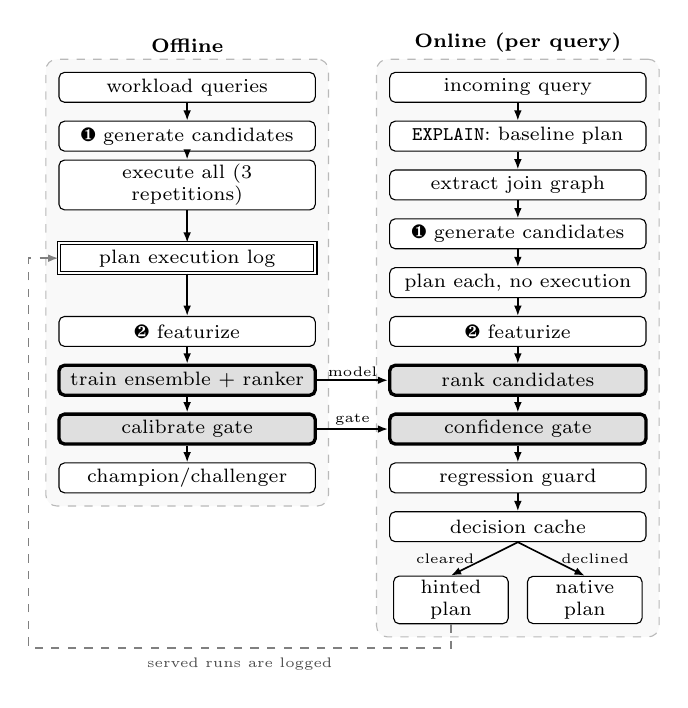
\begin{tikzpicture}[
  font=\scriptsize,
  box/.style={draw, rounded corners=2pt, fill=white, text width=3.15cm,
              align=center, minimum height=0.38cm, inner sep=1.5pt},
  learned/.style={box, fill=gray!25, very thick},
  store/.style={box, rounded corners=0pt, double, double distance=0.8pt},
  arr/.style={-{Latex[length=1.3mm]}, semithick},
  lane/.style={draw=gray!55, dashed, rounded corners=4pt, fill=gray!5,
               inner sep=0.16cm},
  lanelabel/.style={font=\scriptsize\bfseries, anchor=south, inner sep=2pt}
]
\def\dy{0.62}
\def\xb{4.2}
% offline path
\node[box]     (a1) at (0,0)        {workload queries};
\node[box]     (a2) at (0,-1*\dy)   {\ding{182}\ generate candidates};
\node[box]     (a3) at (0,-2*\dy)   {execute all (3 repetitions)};
\node[store]   (a4) at (0,-3.5*\dy) {plan execution log};
\node[box]     (a5) at (0,-5*\dy)   {\ding{183}\ featurize};
\node[learned] (a6) at (0,-6*\dy)   {train ensemble + ranker};
\node[learned] (a7) at (0,-7*\dy)   {calibrate gate};
\node[box]     (a8) at (0,-8*\dy)   {champion/challenger};
% online path
\node[box]     (b1)  at (\xb,0)      {incoming query};
\node[box]     (b2)  at (\xb,-1*\dy) {\texttt{EXPLAIN}: baseline plan};
\node[box]     (b3)  at (\xb,-2*\dy) {extract join graph};
\node[box]     (b4)  at (\xb,-3*\dy) {\ding{182}\ generate candidates};
\node[box]     (b5)  at (\xb,-4*\dy) {plan each, no execution};
\node[box]     (b6)  at (\xb,-5*\dy) {\ding{183}\ featurize};
\node[learned] (b7)  at (\xb,-6*\dy) {rank candidates};
\node[learned] (b8)  at (\xb,-7*\dy) {confidence gate};
\node[box]     (b9)  at (\xb,-8*\dy) {regression guard};
\node[box]     (b10) at (\xb,-9*\dy) {decision cache};
\node[box, text width=1.35cm] (b11) at ({\xb-0.85},-10.5*\dy) {hinted plan};
\node[box, text width=1.35cm] (b12) at ({\xb+0.85},-10.5*\dy) {native plan};
% flow within each path
\foreach \u/\v in {a1/a2,a2/a3,a3/a4,a4/a5,a5/a6,a6/a7,a7/a8}
  \draw[arr] (\u) -- (\v);
\foreach \u/\v in {b1/b2,b2/b3,b3/b4,b4/b5,b5/b6,b6/b7,b7/b8,b8/b9,b9/b10}
  \draw[arr] (\u) -- (\v);
\draw[arr] (b10.south) -- node[left, font=\tiny] {cleared} (b11.north);
\draw[arr] (b10.south) -- node[right, font=\tiny] {declined} (b12.north);
% artifacts handed from offline to online
\draw[arr] (a6.east) -- node[above, font=\tiny, inner sep=1pt] {model} (b7.west);
\draw[arr] (a7.east) -- node[above, font=\tiny, inner sep=1pt] {gate} (b8.west);
% feedback
\draw[arr, dashed, gray] (b11.south) -- ++(0,-0.3)
  -| node[pos=0.25, below, font=\tiny, text=black!70] {served runs are logged}
  ($(a4.west)+(-0.38,0)$) -- (a4.west);
% lanes
\begin{scope}[on background layer]
  \node[lane, fit=(a1)(a8)] (laneA) {};
  \node[lane, fit=(b1)(b11)(b12)] (laneB) {};
\end{scope}
\node[lanelabel] at (laneA.north) {Offline};
\node[lanelabel] at (laneB.north) {Online (per query)};
\end{tikzpicture}
\caption{Offline training and online serving paths. Shaded boxes are learned or
calibrated; the others perform enumeration and bookkeeping. The offline path
produces the model and the gate configuration consumed online. The steps marked
\protect\ding{182} (candidate generation) and \protect\ding{183} (featurization) are implemented
separately on each path and were never compared automatically. Both diverged:
collection explored a wider candidate space than serving offered, and a
\texttt{has\_hint} feature that separated baselines from candidates offline was
constant online (Section~\ref{sec:q2}).}
\label{fig:pipeline}
\end{figure}

\subsection{Candidate Generation}

Our first generator sampled join orders uniformly from all permutations, and
most of what it produced was useless. An order that introduces a table sharing
no join predicate with those already joined forces a Cartesian product, which
PostgreSQL costs at around $10^{10}$ and never chooses. Reading the join graph
from the \texttt{Hash Cond}, \texttt{Merge Cond} and \texttt{Index Cond} entries
of the baseline plan and generating only connected orders raised the usable
fraction on our three- and four-table queries from 23 of 48 (48\%) to 40 of 40.
On one query the blind generator had produced a single usable candidate out of
eight, leaving it with effectively no action space.

\subsection{Features}

Each candidate is a fixed-length vector: per-table slots recording join
position, estimated selectivity and whether the table is read through an index
scan, plus tree-level aggregates and the planner's cost estimate. Slots are
indexed by table rather than by alias and aggregate over repeated occurrences.
Our first implementation assigned them instead, so in a self-join, which JOB
uses routinely, the second occurrence of a table silently overwrote the first.

\subsection{Model and Gate}
\label{sec:gate}

The model is a bootstrapped ensemble of eight LightGBM~\cite{lightgbm}
regressors, each trained to predict a candidate's latency as a log-ratio to the
native plan, so the ensemble gives a mean $\mu$ and a standard deviation
$\sigma$ for every candidate. A separate LightGBM classifier, trained on pairs
of candidates from the same query, serves as the pairwise ranker. Once a
selection policy has picked a candidate, the gate decides whether to serve it in
place of the native plan. It deviates only if both
\begin{equation}
e^{\mu} < 1 - g\kappa
\quad\text{and}\quad
e^{\mu + z\kappa\sigma} < 1 + \frac{\rho - 1}{\kappa},
\label{eq:gate}
\end{equation}
where $g$ is the minimum relative gain, $z$ the confidence multiplier, $\rho$
the largest tolerated slowdown relative to native (1.25 by default) and
$\kappa \ge 1$ a caution factor supplied by the regression guard. The first test
asks whether there is an expected win, and the second whether the plausible
downside is bounded. In an alternative mode, the bound replaces $z\sigma$ with
a quantile of the ensemble's out-of-bag residuals, an idea borrowed from
conformal prediction~\cite{vovk}. We treat this as an empirical residual-based
bound and claim no coverage guarantee for it: our procedure does not meet the
conditions such guarantees require, and across ten splits its measured coverage
ranged from 62.5\% to 92.6\% against a nominal 90\%.

Four selection policies are implemented (greedy, Thompson sampling, risk-averse
and pairwise ranking), along with a Borda aggregation of the orderings produced
by the ensemble and the ranker. Pairwise ranking is the default because it
measured best, not for any reason of principle.

\subsection{Deployment Machinery}

New models enter service through a champion/challenger comparison on a
held-out split and can be rolled back. A regression guard blocks a hint family on any query where that
family has repeatedly regressed. For a query with no served history it also
sets the caution factor $\kappa$ in~\eqref{eq:gate} to 2.0, which tightens both
tests, and eases it toward 1.0 as history accumulates. Served decisions are cached per query template. We describe
this machinery because it shaped the rest of the paper. Several of the defects
in Section~\ref{sec:failures} arose because one component was written for the
offline path and a second, slightly different one for the serving path.

%% ===========================================================================
\section{Experimental Setup}
\label{sec:setup}

\subsection{Platform}

All experiments run on a single machine (Intel Core Ultra~7 155H with 16 cores
and 22 hardware threads, 32\,GB of RAM, NVMe SSD, Windows~11), with
PostgreSQL and \texttt{pg\_hint\_plan} built from source inside a Docker
Desktop container; the current versions are PostgreSQL~18.6 and
\texttt{pg\_hint\_plan}~1.8.1. Apart from the preloaded extensions described below
and the \texttt{compute\_query\_id} and \texttt{track\_io\_timing} settings,
the server runs with its default configuration. The optimizer is written in
Python (FastAPI, psycopg2 and LightGBM) and connects to the database as an
ordinary client. Both \texttt{pg\_hint\_plan} and
\texttt{pg\_stat\_statements} are preloaded at server start. This detail is
itself an instance of the failures studied here: if \texttt{pg\_hint\_plan} is
only installed with \texttt{CREATE EXTENSION}, hints are accepted and silently
ignored, and every candidate collapses to the default plan. Candidate plans are
executed one at a time, never concurrently, so that they do not compete for CPU
time and shared buffers. The project moved from PostgreSQL~16 to~18 partway
through. Figures from its early history, including the synthetic and TPC-H
ceilings in Table~\ref{tab:ceiling}, the 18.6\% noise figure of
Section~\ref{sec:noise} and the candidate-generation counts of
Section~\ref{sec:system}, were measured before the upgrade. The corrections of
Section~\ref{sec:corrections}, the action-space sweep and the cold-start replay
were measured on PostgreSQL~18.

JOB figures, including the transfer results, are computed from logged
collection runs, in which each candidate is executed three times and the median
is kept. The synthetic-workload timing results (Table~\ref{tab:paired}) use
the live protocols of Section~\ref{sec:timing}, and the end-to-end measurement
of
Section~\ref{sec:survives} times live requests from the client.

\subsection{Workloads}

We use three workloads.

\subsubsection{Synthetic Workload}
We use a six-table e-commerce schema with about 755k rows, built
deliberately with correlated columns (city determines country, brand determines
category, and price band and channel are correlated with category and order
status) so that PostgreSQL's independence assumption misestimates conjunctive
predicates. An earlier version of the schema without these correlations (v1,
25 queries) offered almost no headroom, as Section~\ref{sec:ceiling} shows. The
current workload has 65 queries joining two to six tables, including
aggregation, \texttt{DISTINCT}, top-$N$, window-function and semi- and
anti-join shapes. Sixteen queries are held out from training.

\subsubsection{Join Order Benchmark}
We also use JOB~\cite{leis,jobrepo} on the IMDB dataset
(21 tables, about 73M rows). We collect the 30 smallest of its 113 queries, the
largest of which joins seven tables, and hold out eight.

\subsubsection{TPC-H}
In this paper we use TPC-H only for its oracle ceiling.

\subsection{Metrics}

For a query $q$, let $\mathcal{A}(q)$ be the action space, i.e., the set of
candidate plans the system may choose from, including PostgreSQL's native plan
$p_{\mathrm{nat}}(q)$. Let $t(q,p)$ be the measured latency of plan $p$ and
$p_{\mathrm{srv}}(q)$ the plan actually served. Over a set of queries $Q$ we
define the native, served and oracle totals
\begin{align}
T_{\mathrm{nat}} &= \textstyle\sum_{q\in Q} t\bigl(q, p_{\mathrm{nat}}(q)\bigr),
\qquad
T_{\mathrm{srv}} = \textstyle\sum_{q\in Q} t\bigl(q, p_{\mathrm{srv}}(q)\bigr),
\nonumber\\
T_{\mathrm{orc}} &= \textstyle\sum_{q\in Q}\ \min_{p\in\mathcal{A}(q)} t(q,p),
\end{align}
and the capture ratio
\begin{equation}
C = \frac{T_{\mathrm{nat}} - T_{\mathrm{srv}}}{T_{\mathrm{nat}} - T_{\mathrm{orc}}}.
\label{eq:capture}
\end{equation}
We call $T_{\mathrm{nat}} - T_{\mathrm{orc}}$ the \emph{headroom} and
$T_{\mathrm{nat}} - T_{\mathrm{srv}}$ the latency \emph{saved}. The notation
makes the central point of this paper explicit: $T_{\mathrm{orc}}$, and with it
$C$, depends on $\mathcal{A}$, which the experimenter chooses. A negative $C$
means the served plans are slower in total than the native ones. Where we report
latencies relative to native, a value above $1.0\times$ is a slowdown.

%% ===========================================================================
\section{Measurement Methodology}
\label{sec:method}

\subsection{The Oracle Ceiling}
\label{sec:ceiling}

For every query we execute every candidate and record the fastest. Up to
measurement noise, this is the best result any plan selector could achieve
within the action space, and we report it beside every ratio. Section~\ref{sec:corrections} shows why. A capture
ratio is a fraction of an opportunity, and without the size of that
opportunity, a narrow action space cannot be told apart from a good model.

Table~\ref{tab:ceiling} gives the ceilings for our workloads. The 6.5\% ceiling
of the first synthetic workload is the most instructive number in the project's
early history. PostgreSQL already chose the best available plan for 18 of its
25 queries, and none of six model families (LightGBM, random forest, extra
trees, gradient boosting, ridge regression and a multilayer perceptron) picked
the fastest plan for a single query. We do not read this as six failed models.
With only seven queries offering more than 5\%, the workload contained very
little to learn. Rebuilding the schema around
correlated columns raised the mean best-possible gain to 22.2\%, and the
largest gains appeared on exactly the correlations we had planted.

\begin{table}[t]
\caption{Oracle Ceilings by Workload}
\label{tab:ceiling}
\centering
\footnotesize
\setlength{\tabcolsep}{4pt}
\begin{tabular}{|l|c|c|c|c|}
\hline
\textbf{Measure} & \makecell{\textbf{Synth.}\\\textbf{v1}} &
  \makecell{\textbf{Synth.}\\\textbf{v2}} & \textbf{TPC-H} & \textbf{JOB} \\
\hline
Mean best-possible gain & 6.5\% & 22.2\% & $\approx$23\% & $\approx$82\% \\
\hline
Queries with $>$5\% gain & 7/25 & 14/23 & ---\textsuperscript{a} & 5/8 \\
\hline
Best top-1 accuracy & 0\% & --- & --- & 38\% \\
\hline
\multicolumn{5}{l}{JOB figures are over its eight held-out queries.}\\
\multicolumn{5}{l}{\textsuperscript{a}A dash means the quantity was not
  measured.}
\end{tabular}
\end{table}

\subsection{Alternated Timing}
\label{sec:timing}

Our original protocol, which we call \texttt{deploy}, ran the native arm, the
served arm and the oracle arm in sequence, each once. This has two problems.
First, any drift between runs, such as a change in cache state, autovacuum
activity or other load on the machine, is attributed to whichever arm happens to
be running at the time. Second, the oracle is a minimum over noisy measurements
and is therefore biased downward. The more candidates are timed, the better the
ceiling looks by chance alone, which inflates the headroom and deflates every
capture ratio computed from it.

The \texttt{paired} protocol (Algorithm~\ref{alg:paired}) keeps the single
enumeration pass for choosing plans but not for reporting them. For each query it re-times the native plan, the served
plan and the plan that was fastest in the enumeration pass, five times by
default, and reports medians. The order of the three arms is shuffled
independently in every repetition, so that no arm is always timed first or
last. (The single runs in Table~\ref{tab:paired} predate this change and used
a fixed order; its five-run replication uses the randomized one.) Drift then affects all three arms
roughly equally, and the oracle is no longer a minimum over single draws of
every candidate. The result is an oracle \emph{estimate}, and its biases run
in both directions. It can be too high, because only the enumeration pass's
fastest plan is re-timed and that plan need not be the fastest in the action
space. It can be too low, because line~12 of Algorithm~\ref{alg:paired} takes
the minimum of three medians, which can pick up a downward fluctuation.
Re-timing every candidate would remove the first bias, at a cost that grows
with the number of candidates per query. Section~\ref{sec:corrections} reports what the protocol did to our
headline result.

\begin{algorithm}[t]
\caption{Paired Timing With an Oracle Estimate}
\label{alg:paired}
\small
\begin{algorithmic}[1]
\Require queries $Q$; action space $\mathcal{A}(q)$; served policy $\pi$;
  repetitions $R$ (default 5)
\Ensure totals $T_{\mathrm{nat}}$, $T_{\mathrm{srv}}$, $T_{\mathrm{orc}}$
\State $T_{\mathrm{nat}}, T_{\mathrm{srv}}, T_{\mathrm{orc}} \gets 0$
\For{each $q \in Q$}
  \State execute each $p \in \mathcal{A}(q)$ once, giving $t_1(p)$
    \Comment{enumeration pass}
  \State $p_{\mathrm{srv}} \gets \pi(q)$;\quad
    $p_{\mathrm{orc}} \gets \arg\min_{p\in\mathcal{A}(q)} t_1(p)$
  \State $S_{\mathrm{nat}}, S_{\mathrm{srv}}, S_{\mathrm{orc}} \gets \emptyset$
  \For{$r \gets 1$ \textbf{to} $R$}
    \For{$a \in \textsc{Shuffle}(\mathrm{nat}, \mathrm{srv}, \mathrm{orc})$}
      \Comment{order randomized}
      \State execute $p_a$ and append its latency to $S_a$
    \EndFor
  \EndFor
  \State $m_a \gets \operatorname{median}(S_a)$ for each arm $a$
  \State $m_{\mathrm{orc}} \gets \min(m_{\mathrm{orc}}, m_{\mathrm{nat}},
    m_{\mathrm{srv}})$ \Comment{oracle estimate $\le$ both arms}
  \State $T_a \gets T_a + m_a$ for each arm $a$
\EndFor
\State \Return $T_{\mathrm{nat}}$, $T_{\mathrm{srv}}$, $T_{\mathrm{orc}}$
\end{algorithmic}
\end{algorithm}

\subsection{The Noise Floor}
\label{sec:noise}

Repeated executions of the same unchanged plan differ by 18.6\% on average on
our setup, and
we treat a latency difference smaller than that as unresolved. This is a single
global figure, not a per-query floor, and noise may well differ from query to
query.

We also tried to obtain per-query floors without extra executions, from logged
candidate plans that reported identical buffer counts, on the reasoning that
such plans had done the same work. We no longer rely on that estimate, for two
reasons. First, equal buffer counts do not imply equal work: two plans can read
the same pages while doing different amounts of CPU work, for example with
different join algorithms, so part of the latency difference between them is
real. Second, PostgreSQL reports each node's buffer counts inclusive of its
children, so the sum over the plan tree that our implementation used
double-counts page accesses. The resulting spreads mix noise with genuine
differences in work. Per-query floors should come from repeated executions of
the same plan, which we have not yet run per query.

%% ===========================================================================
\section{A Taxonomy of Silent Failures}
\label{sec:failures}

We organize the defects by the question that exposed them, roughly in the order
in which we learned to ask each one. Table~\ref{tab:questions} lists the seven
questions with representative defects and their measured cost. Several defects
were caught before they reached a reported figure and cost nothing, which is
the best argument for asking these questions routinely instead of waiting for a
surprising result.

\begin{table*}[t]
\caption{The Seven Audit Questions, Representative Defects Each One Found, and
What Those Defects Cost}
\label{tab:questions}
\centering
\footnotesize
\setlength{\tabcolsep}{4pt}
\begin{tabular}{|l|p{7.2cm}|p{4.4cm}|}
\hline
\textbf{Audit Question} & \textbf{Representative Defect} &
  \textbf{Measured Cost} \\
\hline
\makecell[l]{\textbf{Q1} Is this code reached?} &
  conformal gate fitted on every run, consulted on none &
  never reached production \\
\cline{2-3}
& \texttt{INCLUDE\_DISABLE\_INDEX} generator gated on a different flag &
  one hint family silently absent \\
\cline{2-3}
& malformed environment variable crashing every entry point at import &
  whole system, from one typo \\
\hline
\makecell[l]{\textbf{Q2} Does this measurement agree\\with what runs?} &
  \texttt{has\_hint} separating baselines from candidates in training &
  8.3 points of held-out capture \\
\cline{2-3}
& benchmark offering plans that the server discards &
  36 of 43 safety vetoes \\
\hline
\makecell[l]{\textbf{Q3} Is this worth building,\\asked before building?} &
  three well-motivated features that changed 0 of 16 decisions &
  the build itself \\
\hline
\makecell[l]{\textbf{Q4} Which population is this\\computed over?} &
  five hint families about to be priced on four held-out queries &
  a misleading 128-arm sweep, avoided \\
\hline
\makecell[l]{\textbf{Q5} At what granularity does\\this rule resolve conflicts?} &
  ``latest run wins'' per query, silently dropping a whole hint family &
  one family: 16 of 16 $\rightarrow$ 0 of 16 queries \\
\hline
\makecell[l]{\textbf{Q6} Is the tool wrong, or the\\thing it measures?} &
  a prefilter blamed for discarding winners; the logged oracle was wrong &
  oracle was a no-op on 11 of 65 queries \\
\hline
\makecell[l]{\textbf{Q7} Which language reads\\this string?} &
  a word-boundary escape read as a backspace by both Python and PostgreSQL &
  a filter that never fired \\
\hline
\end{tabular}
\end{table*}

\subsection{Q1: Is This Code Reached?}
\label{sec:q1}

This was the most common failure and, taken one at a time, the least
interesting. Examples include a conformal gate that was fitted on every training
run and consulted on none; a swept \texttt{gate\_mode} parameter that the API
ignored; a configuration flag with six lines of documentation and no effect;
39\% of the action space assigned to a catch-all category and dropped from every
replay; and a hint family whose candidate generator checked a different flag
from the one that enabled it, so that it produced no candidates at all.

One recent instance shows how far such a defect can reach. We had a documented
policy that a malformed environment variable should never prevent the server
from starting. The policy could not take effect, because the learner module
parsed five floating-point variables with a bare \texttt{float()} call at
import time, and the settings module, which implemented the policy, imported
the learner. A single malformed value therefore crashed every entry point in
the system, including the component whose job was to prevent exactly that.
Unlike most defects here, this one was loud once triggered, but it stayed latent
until a malformed value arrived. An audit afterwards found seven more variables
parsed the same way at import, in four other modules.

\subsection{Q2: Does This Measurement Agree With What Runs?}
\label{sec:q2}

This family is train/serve skew in the broad sense, and it cost us more than
any other. Instances include gate calibrations that all measured a selection
policy the server did not run; a calibration sweep that scored an action space
narrower than the one being served; a drift check that judged a newly applied
gate by the runs served under its predecessor; a benchmark that offered the
model plans containing disabled nodes,
which the server always discards, accounting for 36 of 43 safety vetoes in one
run; and data collection that explored a wider candidate space than serving
ever offered, so that 14.4\% of logged candidates were plans byte-identical to
the native one. On 11 of the 65 queries, one of these duplicates had been
recorded as the oracle.

A boolean feature recording whether a candidate carried any hint also belongs
here. It was perfectly discriminative in training, because it separated the 65
baseline rows from the 2,257 candidate rows. At serving time the ranker sees
only candidates, every one of which carries a hint, so the feature is constant. Removing it improved held-out capture by a mean of 8.3 points
across 16 splits, better on 11 of them. Our own notes had earlier credited that
gain to dropping all 23 features that are constant within a query. On
re-checking, the other 22 made no difference on any of the 16 splits, and the
whole effect came from this one feature. An ablation that removes a group of
features and credits the group with the result is really measuring the group's
most consequential member. The resulting model was nevertheless refused at
promotion, because its worst pick was $3.31\times$ the best available plan
against the incumbent's $1.41\times$.

\subsection{Q3: Is This Worth Building, Asked Before Building?}
\label{sec:q3}

Asking this question first was cheap and effective. Before writing one proposed
feature we checked that it increased monotonically with available headroom. We
measured another proposed signal, from \texttt{pg\_overexplain}, at a median
within-query rank correlation of $+0.04$ with latency over 56 queries, which is
indistinguishable from chance, and never built it. We rejected buffer counts as
a training label because of their 0.341 rank correlation with latency.

The question has a second half that we learned the hard way. Three features we
did build, on good evidence, changed the model's choice on none of the 16
held-out queries. The evidence was sound but measured along the wrong axis. The
features predict which \emph{queries} have headroom, whereas our ranker compares
\emph{plans within one query}, and any query-level feature is constant within a
query. The useful form of the question is therefore whether a component is worth
building when measured against what that component actually decides.

\subsection{Q4: Which Population Is This Computed Over?}
\label{sec:q4}

Two of our components answered ``is this feature constant?'' over different
rows, one over candidates only and the other over candidates and baselines
together, and the one that acted on its answer could not see the only feature
worth removing.

A later instance has a practical corollary. Before pricing five newly collected
hint families with a sweep over all 128 combinations of optional families, we
asked which population it would be computed over. The collection had been
interrupted after 16 of the 65 queries, all from the correlated-predicate family
that the workload lists first, and only four of those 16 were in the held-out
split the sweep scores. The families' measured differences on those four
queries ($-15$, $-7$, $0$, $0$ and $+2$\,ms) were well inside the noise floor,
yet the sweep would have ranked them to the millisecond without saying so. The
collection budget and the evaluation population have to be chosen together. Ours
lived in different modules, and nothing ever multiplied the two fractions.

\subsection{Q5: At What Granularity Does This Rule Resolve Conflicts?}
\label{sec:q5}

Our fix for the previous defect introduced a new one. We re-collected the 16
held-out queries with the five families under investigation enabled. Afterwards
those families covered all 16 queries, but \texttt{scan\_method}, present on all
65 queries an hour earlier, covered none of them, although all 43,327 rows were
still in the log. The replay keeps only the most recent collection run for each
query, so that a candidate measured in one run is never compared with a native
plan measured in another (the same native query had ranged from 2.4\,ms to
13.7\,ms across runs). That rule is right, but it operates per query, so
superseding a query also superseded every family in it, and our re-collection
had not enabled \texttt{scan\_method}. The sweep derives its axes from the data
and would have silently swept six optional families instead of seven.

A conflict-resolution rule chosen at one granularity applies to everything
nested beneath it. ``Latest run wins'' was also a decision about families, and it
made a narrower collection destructive rather than additive. We caught it only
because two functions, one reading the full history and the other the latest
run, reported different coverage for the same family (65 and 33 queries).
Collection now warns before it narrows the family set of the run it supersedes.

\subsection{Q6: Is the Tool Wrong, or the Thing It Measures?}
\label{sec:q6}

Three times, the first reading attributed to the system what was really a
property of the instrument. A gate that appeared badly calibrated was being
evaluated on candidates the server would discard. A prefilter that appeared to
discard winning plans on 10 of the 62 queries with a real win was correct:
re-planned with and without those hints, none of the ten plans changed, and the
apparent wins were timing differences between identical plans, so it was the
log's oracle that was wrong. And a transfer result read as evidence that the
model generalized reflected the narrow candidate set it was measured on
(Section~\ref{sec:corrections}).

\subsection{Q7: Which Language Reads This String?}
\label{sec:q7}

This is the narrowest question, and the only one not about the seams between
our own components. A regular expression meant to exclude \texttt{BEGIN},
\texttt{COMMIT}, \texttt{SET} and similar statements from a workload report was
written in a non-raw Python string, so its word-boundary escape \verb|\b| became
a backspace and the filter never excluded a row. Python warned about a
different, harmless escape in the same pattern. Making the string raw does not
fix it either, because PostgreSQL's regular expressions also read \verb|\b| as a
backspace; the word boundary there is \verb|\y|. A pattern written in one
language and executed by another has every escape interpreted twice, and a
warning from the outer language says nothing about the inner one.

%% ===========================================================================
\section{Results}
\label{sec:results}

\subsection{Three Corrections}
\label{sec:corrections}

Table~\ref{tab:corrections} lists the three previously reported figures that did not
survive the audit. In all three cases the model itself was unchanged.

\begin{table}[t]
\caption{Headline Results Before and After Correction}
\label{tab:corrections}
\centering
\footnotesize
\setlength{\tabcolsep}{3pt}
\begin{tabular}{|l|c|c|l|}
\hline
\textbf{Claim} & \textbf{Before} & \textbf{After} & \textbf{Cause of Change} \\
\hline
JOB headroom captured & 99.2\% & 91.0\% & wider space; drift \\
\hline
Synthetic latency saved & 797\,ms & 215\,ms\textsuperscript{b} & paired timing \\
\hline
Cross-schema transfer\textsuperscript{a} & 97.0\% & $-5.3$\% &
  wider candidate set \\
\hline
\multicolumn{4}{p{0.94\columnwidth}}{\scriptsize \textsuperscript{a}Capture
ratio of a model trained on the synthetic schema. \textsuperscript{b}Five
randomized runs: mean 84\,ms, 95\% CI [$-226$, 393] (Table~\ref{tab:paired}). No
model was retrained between the two columns.}
\end{tabular}
\end{table}

\subsubsection{JOB Capture Ratio}
Re-collecting all 30 JOB queries under the wider action space
took 8\,h 22\,min. On the eight held-out queries the oracle's total latency fell
from 696\,ms to 520\,ms, while the plans our model served went from 723\,ms to
718\,ms (Fig.~\ref{fig:job}). The uncaptured gap
$T_{\mathrm{srv}} - T_{\mathrm{orc}}$ therefore grew from 27\,ms to 198\,ms. We
attribute most of the 176\,ms fall in the oracle to plans that only the wider
space contains, although the two runs also differ in machine state; in either
case the model's served total barely moved. The capture ratio fell from 99.2\%
to 91.0\%.

Not all of that drop is due to the action space. The native total for the same
eight queries also changed between the two runs, from 3,960\,ms to 2,715\,ms, a
31\% change with no change to the queries or the data. As an illustrative
sensitivity calculation, holding the native total fixed at either run's value
attributes between 5.0 and 7.7 of the 8.2 points to the wider space. This is
not a clean attribution, because the served and oracle totals were also timed
in different runs and may have drifted too. A controlled comparison would time
both action spaces within the same run. The drift is also why we compare arms
only within a single run, and why we lean on the uncaptured gap, which does not
involve the native total, though it is not immune to drift either.

\begin{figure}[t]
\centering
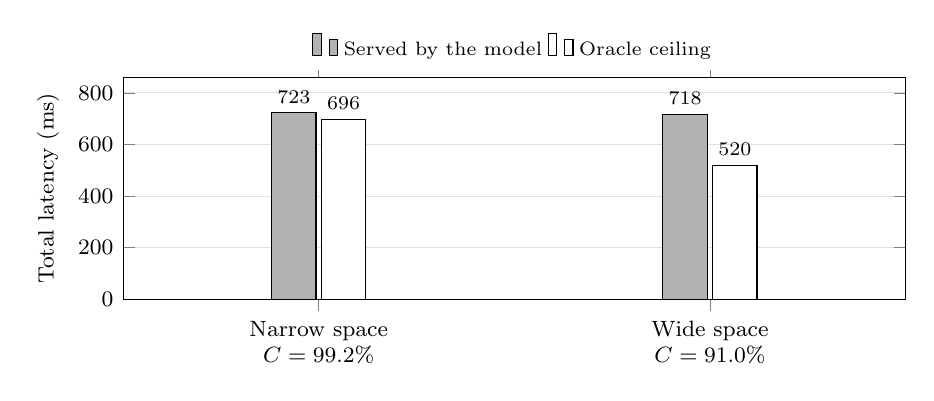
\begin{tikzpicture}
\begin{axis}[
  ybar, bar width=16pt,
  width=0.95\columnwidth, height=4.4cm,
  ymin=0, ymax=860,
  ylabel={Total latency (ms)},
  ylabel style={font=\footnotesize},
  symbolic x coords={narrow,wide},
  xtick=data,
  xticklabels={{Narrow space\\$C=99.2\%$},{Wide space\\$C=91.0\%$}},
  xticklabel style={align=center, font=\footnotesize},
  yticklabel style={font=\footnotesize},
  enlarge x limits=0.5,
  nodes near coords,
  nodes near coords style={font=\scriptsize},
  legend style={at={(0.5,1.03)}, anchor=south, legend columns=2,
                font=\scriptsize, draw=none},
  ymajorgrids, grid style={gray!25},
]
\addplot[fill=gray!60, draw=black] coordinates {(narrow,723) (wide,718)};
\addplot[fill=white, draw=black] coordinates {(narrow,696) (wide,520)};
\legend{Served by the model, Oracle ceiling}
\end{axis}
\end{tikzpicture}
\caption{Served and oracle totals on the eight held-out JOB queries under the
narrow and wide action spaces, from two separate collection runs. The oracle
fell by 176\,ms while the served plans changed by 5\,ms, so the uncaptured gap
grew from 27\,ms to 198\,ms with no change to the model. Native totals (3,960\,ms and
2,715\,ms) are omitted for scale. They differ because of between-run drift,
which also affects $C$.}
\label{fig:job}
\end{figure}

\subsubsection{Timing Protocol}
Table~\ref{tab:paired} compares the \texttt{deploy} and
\texttt{paired} protocols on the same code and the same gate, within the same
hour; only the timing differs. Every arm is faster under the \texttt{paired}
protocol, which is consistent with warmer caches once each plan is executed
repeatedly. The two protocols therefore also measure somewhat different cache
regimes, and part of the difference between them may reflect cache state
rather than noise alone. With that caveat, the measured headroom shrinks by
66\% and the latency actually saved shrinks by 73\%. The capture ratio~\eqref{eq:capture} also falls, from
61.1\% to 48.1\%, so
the correction does not merely shift the flattery from one metric to another.

\begin{table}[t]
\caption{Timing Protocols on the 65-Query Synthetic Workload}
\label{tab:paired}
\centering
\footnotesize
\setlength{\tabcolsep}{3pt}
\begin{tabular}{|l|c|c|c|}
\hline
 & \multicolumn{2}{c|}{\textbf{One run}} & \textbf{5 random runs} \\
\textbf{Quantity} & \texttt{deploy} & \texttt{paired} & \textbf{mean [95\% CI]} \\
\hline
Native (ms) & 7,426 & 5,680 & 6,120 [5,912, 6,328] \\
Served (ms) & 6,629 & 5,464 & 6,036 [5,569, 6,503] \\
Oracle (ms) & 6,122 & 5,232 & 5,594 [5,441, 5,748] \\
\hline
Headroom (ms) & 1,304 & 448 & 526 [452, 599] \\
Saved (ms) & 797 & 215 & 84 [$-226$, 393] \\
Saved (\% of native) & 10.7 & 3.8 & 1.4 [$-3.7$, 6.5] \\
Captured, $C$ (\%) & 61.1 & 48.1 & 17.4 [$-41.7$, 76.6] \\
\hline
Held-out saved (ms) & 85 & 12 & $-13$ [$-45$, 19] \\
Held-out $C$ (\%) & 40.0 & 18.4 & $-19.4$ [$-72.8$, 34.0] \\
\hline
\multicolumn{4}{p{0.94\columnwidth}}{\scriptsize The single runs used a fixed
arm order; the five runs randomized it and used a database restored from a
4~September 2026 backup. Intervals use Student's $t$ with four degrees of
freedom. Derived rows use unrounded totals, so they can differ by 1\,ms from
differences of the rounded rows.}
\end{tabular}
\end{table}

\subsubsection{Replication With Randomized Arm Order}
The single \texttt{paired} run used a fixed arm order. To see how stable it is,
we repeated the \texttt{paired} protocol five times with the arm order
randomized (Algorithm~\ref{alg:paired}) and a different seed for each run,
using the current model and gate on PostgreSQL~18.6, with the database restored
from a backup taken on 4~September 2026. The last column of
Table~\ref{tab:paired} gives the mean of each quantity and a 95\% confidence
interval from Student's $t$ distribution with four degrees of freedom.

The headroom is stable: 526\,ms on average, with an interval from 452 to
599\,ms, close to the 448\,ms of the single paired run. The saving is not. Its
mean is 84\,ms, 1.4\% of native, and its interval runs from $-226$ to
$+393$\,ms, so these five runs cannot distinguish the system's effect on this
workload from zero. Captured headroom ranged from $-37.2$\% to $64.3$\% across
the runs. On the 16 held-out queries the mean saving was $-13$\,ms, with an
interval from $-45$ to $+19$\,ms.

The runs are also not independent. Each run logs its executions and the
regression guard reads that log, so the guard blocked no queries in the first
three runs and 11 and 12 queries in the last two, once the earlier runs had
recorded regressions. The first three runs lost 69\,ms on average and the last
two saved 312\,ms. Five runs cannot separate that from run-to-run noise, but the
pattern suggests that much of whatever benefit the system delivers here comes
from the guard declining to deviate on queries where deviation has already
failed, rather than from better choices.

\subsubsection{Cross-Schema Transfer}
This was our strongest claim to external validity. A model
trained on the six-table synthetic schema and applied to JOB, with no tables in
common and therefore every per-table feature slot reading zero, had captured
97.0\% of JOB's headroom. Table~\ref{tab:transfer} gives the totals before and
after the action space was widened.

A change in the oracle alone cannot change the sign of $C$, and the sign did not
change for that reason. It changed because the transferred model's own choices
got worse: its served total went from 28.1\% of native to 104.0\%, i.e., 4\%
slower than not deviating at all. No model was retrained; the set of candidates
it chose from was wider. Random selection stayed at about the same ratio to
native under both spaces (126.2\% and 125.8\%), so the average candidate did not
get worse; the transferred model's choices did. We have not isolated which of
the added candidates it misranks. The JOB-trained model, shown for reference,
was evaluated on the same queries, which include its own training queries, so
its 96.5\% is not an out-of-sample figure. What the table does show is that the
claim that the schema-independent half of the feature vector is enough on its
own does not survive. The transferred model still ranks plans far better than
chance, but not better than PostgreSQL.

\begin{table}[t]
\caption{Cross-Schema Transfer to JOB, Before and After Widening the Action
Space}
\label{tab:transfer}
\centering
\footnotesize
\begin{tabular}{|l|c|c|}
\hline
\textbf{Total latency (s)} & \textbf{Narrow} & \textbf{Wide} \\
\hline
Native, $T_{\mathrm{nat}}$ & 116.4 & 104.2 \\
Oracle, $T_{\mathrm{orc}}$ & 30.1\textsuperscript{a} & 24.8 \\
Random pick & 147.0 & 131.1 \\
Transferred model, served & 32.7 & 108.4 \\
JOB-trained model, served & 31.5 & 27.5 \\
\hline
Transferred model, $C$ & 97.0\% & $-5.3$\% \\
JOB-trained model, $C$ & 98.4\% & 96.5\% \\
\hline
\multicolumn{3}{l}{\textsuperscript{a}Derived from the recorded native and
  served totals and $C$.}\\
\multicolumn{3}{l}{The JOB-trained model's figures include its training
  queries.}
\end{tabular}
\end{table}

\subsection{Ensemble Uncertainty Measured the Wrong Quantity}
\label{sec:sigma}

Our gate needs an uncertainty estimate for each prediction. The obvious source
is ensemble disagreement: train eight members on bootstrap samples and take the
standard deviation of their predictions. This is what we built, and it was off
by about a factor of four. On the ensemble's own out-of-bag predictions, the
members' typical disagreement was 0.026, while the model's actual error was
0.106. A one-sigma margin was therefore about a quarter of the real uncertainty,
and a gate that required a gain of $z\sigma$ was demanding roughly a quarter of
what it appeared to demand, on every decision it made.

We tried two repairs and measured both. Giving the members different random
seeds changed nothing, to sixteen decimal places. With
\texttt{subsample=1.0} and \texttt{colsample\_bytree=1.0}, LightGBM is
deterministic and the seed has nothing to act on. Enabling row and column
sampling, so that the seed would matter, made the understatement worse (from
$4.04\times$ to $4.41\times$) and slightly weakened the correlation between
$\sigma$ and the actual error (from $+0.238$ to $+0.218$). We reverted both.

Both repairs assumed that the members were too similar to one another. We
believe the real problem is that they all make the same mistake. Ensemble
spread measures variance: how much the model would change if it had been
trained on different data. Under bias, every member errs in the same direction,
so the members agree with each other while all being wrong, and no
rearrangement of the ensemble can reveal an error that none of its members
contains. Our evidence that the error is dominated by bias and by measurement
noise is indirect: two changes that increased the members' diversity did not
narrow the gap, and $\sigma$ correlates only weakly with the actual error. We
have not performed a formal bias--variance decomposition.

The remedy is to estimate uncertainty from how wrong the model has actually been
instead of from how much its members disagree. Conformal
prediction~\cite{vovk} does this, with coverage guarantees that hold under
exchangeability when the procedure is followed as specified, and Liu et
al.~\cite{conformallqo} develop it carefully for learned optimizers. Our own
residual-based bound (Section~\ref{sec:gate}) follows the idea but not the
procedure, and its coverage fell short of nominal on most splits (median
75.5\% against a nominal 90\%). The mistake is easy to make because an
ensemble's standard deviation is a plausible number in the right units that
comes for free. Any system that gates on it should check the ratio of spread to
realized error first.

\subsection{What the Action Space Is Worth}
\label{sec:actionspace}

The preceding sections argue that narrowing an action space flatters the ratio
computed against it. The complementary question is what widening one buys. Our
optimizer has seven optional hint families in addition to the three it always
serves (join order, operator toggles and cardinality correction). Collecting all
seven on the queries our sweep scores took three attempts and exposed the
defects described under Q4 and Q5. With the data finally complete, we swept all
$2^7 = 128$ action spaces under the served policy, replaying logged executions
on the 16 held-out queries. A space survives if its calibrated gate keeps the
share of deviations that regress at or below 25\% and no query slower than
$1.25\times$ native. Table~\ref{tab:spaces} lists every distinct outcome among
the surviving spaces.

\begin{table}[t]
\caption{Distinct Outcomes Among Action Spaces Whose Gate Cleared the Safety
Bounds (128 Swept; Replay on 16 Held-Out Queries)}
\label{tab:spaces}
\centering
\footnotesize
\setlength{\tabcolsep}{3pt}
\begin{tabular}{|l|c|c|c|c|c|}
\hline
\textbf{Extra Families} & $\boldsymbol{z}$ &
  \textbf{Deviates}\textsuperscript{a} & \textbf{Regress}\textsuperscript{b} &
  \textbf{Worst}\textsuperscript{c} & \textbf{Net}\textsuperscript{d} \\
\hline
\emph{none} & 1.00 & 94\% & 20\% & 1.15$\times$ & \textbf{8.7\%} \\
\texttt{bushy} & 1.00 & 94\% & 20\% & 1.15$\times$ & \textbf{8.7\%} \\
\texttt{memoize} & 1.50 & 75\% & 17\% & 1.15$\times$ & 8.1\% \\
\texttt{bushy,memoize} & 1.50 & 75\% & 17\% & 1.15$\times$ & 8.1\% \\
\texttt{resource} & 2.00 & 62\% & 20\% & 1.15$\times$ & 6.1\% \\
\texttt{join\_method} & 2.00 & 62\% & 20\% & 1.00$\times$ & 6.0\% \\
\hline
\multicolumn{6}{p{0.92\columnwidth}}{\scriptsize
\textsuperscript{a}Share of queries on which the gate departs from the native
plan. \textsuperscript{b}Share of those deviations that are slower than native.
\textsuperscript{c}Largest served-to-native latency ratio.
\textsuperscript{d}Net latency improvement over native. Every other surviving
space adds \texttt{bushy} and/or \texttt{memoize} to a row shown and produces
identical numbers.}
\end{tabular}
\end{table}

In this replay, the best space is the three always-on families alone. None of the seven
optional families improves on it, and the net improvement never rises when a
family is added. Three families (\texttt{scan\_method}, \texttt{parallel} and
\texttt{disable\_index}) appear in no surviving space: every space containing
any of them failed the bounds outright.

Most of Table~\ref{tab:spaces}, however, is not a result. The spread among the
survivors is 2.7 points (8.7\% to 6.0\%), while two three-run benchmarks of an
identical configuration once landed 8 points apart, so we report the table but
not a ranking. Two observations are less sensitive to small differences, though
neither is immune to noise. Every space containing \texttt{bushy} produced the
same values as the same space without it, which suggests, though we have not
confirmed it from the selection logs, that no bushy candidate was ever selected.
And the three families that appear in no surviving space failed our replay
safety criteria on this workload, which is not proof that they are unsafe. The
sweep is a replay over logged rows, and its figures should be confirmed under
the \texttt{paired} protocol before being relied on.

\subsection{A Negative Result on Cold Start}
\label{sec:coldstart}

Replayed over the 65-query synthetic log, a fresh installation with no trained
model deviated on every query and ran at $1.040\times$ native latency, with a
worst case of $5.32\times$. The obvious repair, deviating only when the
planner's cost estimate favors the candidate, ran at $1.109\times$ native in the
same replay, with 10 of its 12 deviations (83\%) regressing. We shipped
native-until-trained instead. The losing option looked like the safe,
conservative change, and we would have accepted it without the measurement.

\subsection{What Survives, End to End}
\label{sec:survives}

On execution time alone, the synthetic result is small and uncertain. The
single paired run of Table~\ref{tab:paired} saved 215\,ms, 3.8\% of native, and
the five randomized runs in the same table put the mean saving at
84\,ms, 1.4\%, with an interval that includes zero. On the eight held-out JOB
queries, where the headroom is much larger, the served plans total 718\,ms
against 2,715\,ms for native, but that figure comes from a logged collection
run and was not timed under the \texttt{paired} protocol.

Execution time also leaves out the cost of choosing. We therefore measured what
a client actually waits for (Table~\ref{tab:e2e}). For each of the 65 synthetic
queries we timed three paths from the client, with rows fetched: the query as
written; the full serving path with no cache, in which every candidate is
planned before the chosen plan runs; and the same path with a warm decision
cache. Each query was timed five times per path, with the order of the paths
shuffled in every repetition, and the median was kept. Shadow sampling was
disabled for the measurement.

Without the cache, planning the candidates cost 3.5\,s across the workload, a
median of 54\,ms per query, and the optimizer made the workload 22.5\% slower
than PostgreSQL on its own. With a warm cache, choosing cost 73\,ms in total
and the workload was 3.1\% faster than native. Nearly all of that difference
comes from the 20 queries on which a hint was served, which went from 3,309\,ms
to 2,944\,ms; on the other 45 queries the two paths were within 1\% of each
other. The interval in Table~\ref{tab:e2e} resamples queries within one
session. It shows how much the result depends on which queries are in the
workload, not how much it would move between sessions, which
Table~\ref{tab:paired} shows can be a lot. Taken together, the two
measurements support a modest claim. On repeat traffic served from the cache,
the system may save a few percent. On the first sight of a query, it costs
about a fifth.

\begin{table}[t]
\caption{End-to-End Latency of the 65 Synthetic Queries, Planning Included}
\label{tab:e2e}
\centering
\footnotesize
\setlength{\tabcolsep}{3pt}
\begin{tabular}{|l|c|c|c|}
\hline
\textbf{Path} & \textbf{Total (ms)} & \textbf{vs.\ Native} &
  \textbf{95\% CI (ms)} \\
\hline
Native & 13,642 & --- & --- \\
No cache & 16,711 & $+22.5$\% & [$+2{,}544$, $+3{,}585$] \\
Warm cache & 13,222 & $-3.1$\% & [$-837$, $-48$] \\
\hline
\multicolumn{4}{p{0.92\columnwidth}}{\scriptsize Client wall-clock time,
median of five repetitions per query and path, path order shuffled per
repetition. Choosing a plan cost 3,487\,ms in total without the cache and
73\,ms with it. A hint was served on 20 of the 65 queries. The interval is a
bootstrap over queries for the difference from native.}
\end{tabular}
\end{table}

Two robustness results hold as far as we tested them. In a stress test with six
reader threads and one refreshing thread, the regression guard served 3.1
million concurrent reads with zero errors. We attribute this to the refresh
rebinding each shared attribute to a fully built object instead of mutating it
in place, a property that was load-bearing yet undocumented until we went
looking for it. A test of this kind cannot prove the absence of races, and one
known window remains: the attributes are rebound one after another, so a reader
can briefly pair a new block list with old observations. And on one four-way
join that we profiled under concurrency, uncached planning stayed between 41\%
and 47\% of the query's execution time from one to eight concurrent planners,
because planning and execution slowed down by similar factors ($2.60\times$ and
$2.43\times$ at eight-way concurrency).

%% ===========================================================================
\section{Discussion}
\label{sec:discussion}

\subsection{What a Capture Ratio Needs}

We began intending to recommend that learned optimizers report the oracle
ceiling, but three of the seven systems in Table~\ref{tab:compare} already do,
so our recommendation is narrower. What is missing is the second half. A ceiling is a statement about an action
space, and outside Kepler's notation that space is not reported in a form that
allows comparison across papers. Our own 99.2\% and 91.0\% come from an
identical model on an identical set of queries, and an illustrative calculation
attributes between 5.0 and 7.7 of the 8.2 points between them to the wider
action space, with drift a plausible source of the rest. Neo shows the same dependence from the opposite direction,
approximating the best possible latency by ``the best query latency seen so far
by the system''. A reference of that kind moves with the system being
evaluated, which makes it hard to read as a fixed ceiling.

The timing column carries a separate lesson. Because it varies independently of
the ceiling column, the two are distinct practices rather than one habit of
care. RELOAD takes the median of six repetitions and adds a $2\sigma$ tolerance
band but reports no ceiling. Kepler reports a well-defined ceiling but estimates
each plan's latency as the minimum of three runs. A minimum over noisy draws is
biased low, and the bias compounds when the ceiling is itself a minimum across
plans. In our own measurements, moving from single-pass timing to alternated
medians removed 66\% of the measured headroom (Table~\ref{tab:paired}). The
downward bias of a minimum is one plausible cause, alongside drift and a warmer
cache under repetition, and we have not separated the three. We do not know how
large the effect would be in Kepler's setting.

We therefore recommend three practices. First, report the ceiling together with a
description of the action space that defines it, detailed enough that someone
else could enumerate the same space. Second, estimate the ceiling with a
statistic that is not a minimum over repeated draws. Our own paired estimate
meets the second only in part, since it still takes a minimum over three
medians. Third, repeat the timing with randomized order and report intervals
across runs. Without the first, a capture ratio cannot be compared across
systems; without the second, it is not stable even within one; and without the
third, a single favorable run can pass for a result. Our own corrected run said
the system saved 215\,ms, and five randomized runs could not distinguish its
saving from zero.

\subsection{Making the Audit Questions Executable}

Each audit question that repeatedly found defects has become a single command,
because a lesson that exists only as advice rarely survives the next deadline.
\texttt{diagnostics} compares the policy, action space and calibration time
recorded with the deployed gate against what is running (Q1, Q2).
\texttt{coverage\_sweep} reports a held-out figure as a range over ten splits:
on our workload, held-out capture ranges from 24.2\% to 89.1\%.
\texttt{feature\_audit} lists features that cannot separate the items a
component compares, which is how three well-motivated features were found to
change no decisions (Q3). \texttt{selection\_effect} estimates how much of a
result comes from the choice of workload; only 6 of 40 randomly generated
queries in our schema offer at least 8\% headroom. \texttt{benchmark
-{}-protocol paired} re-times the arms in randomized order and reports intervals
across repeated runs, \texttt{e2e\_latency} counts the cost of choosing against
what it saves, and \texttt{collect\_data -{}-held-out} spends the collection
budget on the queries the sweep can score and warns before narrowing a family
set (Q4, Q5). None of these tools is sophisticated. Their value is that each is
one command, so the question gets asked at inconvenient moments and not only
when someone is already suspicious.

%% ===========================================================================
\section{Threats to Validity}
\label{sec:threats}

\subsubsection{Workload Size}
Our synthetic workload is small, and its held-out split
is smaller still, at 16 of 65 queries. Across ten random splits, held-out
capture varies over a range of 64.9 points, so no single split's figure should
be quoted on its own. This is a sampling problem, and neither more repetitions
nor better timing can fix it. We therefore rely on JOB for our most important
claims. Our JOB collection, however, covers only the 30 smallest of 113 queries,
the largest of which joins seven tables. Twenty of the 113 reach PostgreSQL's
genetic-optimizer threshold (\texttt{geqo\_threshold} $= 12$), so the genetic
optimizer has never planned a query we measured. All of our conclusions concern
the dynamic-programming planner.

\subsubsection{Measurement Resolution}
The single runs in Table~\ref{tab:paired} used a fixed arm
order. The five randomized runs that replicate them are few, and they are not
independent, because the regression guard learns from each run's executions.
Their intervals are correspondingly wide, and they used a database restored
from an earlier backup, so they are not an exact repeat of the single runs'
conditions. On one
earlier occasion, two independent three-run benchmarks of an identical
configuration landed 8 points apart; we take that as a warning about the
instrument's resolution, not as a calibrated bound.

\subsubsection{End-to-End Latency}
The end-to-end measurement of Table~\ref{tab:e2e} is a single session on one
machine, with the client on the same host. Its interval resamples queries, not
sessions. The cached path assumes repeat traffic within the cache's lifetime,
and the measurement excludes shadow sampling and the runtime deadline that the
serving path applies to long-running deviations.

\subsubsection{Baselines}
We compare against PostgreSQL's native plan, the
cost-estimate argmin and random selection, but not against reimplementations of
Bao or Lero. Our results describe one hint-based system and should not be read
as measurements of those systems.

\subsubsection{Environment}
All measurements are single-node and single-instance, on
one machine. We tested the regression guard and the planning path under
concurrency, but not the full serving path; the HTTP layer, the connection pool
and the decision cache under contention remain untested.

\subsubsection{Completeness}
This paper reports more than thirty defects and offers no
evidence that the rate at which we find them is falling. The count should be
treated as a lower bound.

%% ===========================================================================
\section{Conclusion}
\label{sec:conclusion}

We built a learned query optimizer, and it works about as well as a careful
measurement says it does, which is less well than our first measurements
suggested. On the synthetic workload, five randomized runs cannot distinguish
its effect on execution time from zero, and end to end it helps only when its
decisions are reused from the cache. None of the corrections came from
retraining the model. Each came
from a specific structural mistake that produced a plausible number, and each
was found by asking a question rather than by observing a failure. We offer the seven audit questions
and the three reporting practices of Section~\ref{sec:discussion} in the hope that
they save others some of the time they cost us. We arrived at both the hard way:
we reported 99.2\%, and the number that replaced it came out of the same code.

\section*{Artifact Availability}

The implementation, the full defect log with per-defect measurements, and the
measurement tools described in this paper are available at
\url{https://github.com/parthkansal823/DB_QueryOptimizer}. The file
\texttt{docs/WRITEUP.md} records more than ninety findings in the order in which
they were made, including those that turned out to be our own errors. Query
definitions are in \texttt{backend/app/workload.py} (synthetic) and
\texttt{data/job/queries} (JOB), and every trained model bundle records the
identifiers of its held-out queries. The raw results of the replication and
the end-to-end measurement are in \texttt{backend/models}. The version described
in this paper is tagged \texttt{icde2027-submission}. The repository also
includes more than 1,600 unit tests and 18 integration tests that check that
hints actually bind.

%% For the camera-ready version, balance the last page's reference columns with
%% \IEEEtriggeratref{N}, placed here, where N is the reference to break before.
\bibliographystyle{IEEEtran}
\bibliography{references}

\end{document}
